\documentclass[9pt,conference,compsocconf, article]{IEEEtran}
\linespread{0.94}

\usepackage{hyperref}
\usepackage{graphicx}	% For figure environment
\usepackage{subfig}
\usepackage{dsfont}
\usepackage{amsmath}
\usepackage{amsfonts}
\usepackage{xcolor}
\usepackage{todonotes}
\usepackage{booktabs}
\usepackage{amssymb}
\usepackage{pifont}
\usepackage{comment}
\graphicspath{{./images/}}

\bibliographystyle{unsrt}
\include{macro}

\newcommand{\cmark}{\ding{51}}
\newcommand{\xmark}{\ding{55}}

\begin{document}
\title{CS-433 Machine Learning - Semantic Segmentation of Centrioles in Human Cells and Assigning Them to Nuclei}


\author{
Authors: Oliver Becker, Antoine Daeniker, Tim Poštuvan\\
Supervisors: Léo Bürgy, Pierre Gönczy \\
\textit{Gönczy Lab -- Cell and Developmental Biology, EPFL, Switzerland}}


\maketitle

\begin{abstract} 

Determination of the number of centrioles is central to better understand their role in cancer since centrosome amplification often occurs in cancer cells. To detect centrioles, we propose an approach based on semantic segmentation of centrioles. Furthermore, we segment nuclei and assign centrioles to them in an unsupervised manner. The assignment is done by defining the problem as minimum weight matching in a bipartite graph with prior greedy matching. This allows us to incorporate domain knowledge that each nucleus can have at most four centrioles. Our approach is also evaluated at all stages, except for nuclei segmentation one. The source code of this project is available on GitHub. \footnote{https://github.com/timpostuvan/segmentation-of-centrioles}


% https://github.com/CS-433/ml-project-2-bravecentrioles

\end{abstract}

\section{Introduction}

Centrioles are small cylindrical organelles found in cells, responsible for cell division. Pairs of centrioles constitute centrosomes which are associated with cancer -- an uncontrolled division of abnormal cells. Therefore, to prevent cancer, cell division is under tight control and depends on the centrioles, correctly placed at the two poles during the division. Any deregulation in the number of centrioles may therefore cause abnormal division. Due to the connection between centriole number and cell division, unraveling the mechanisms of centriole formation helps understand the circumstances by which cancers form. According to Gönczy \cite{gonczy2015centrosomes}, this fact has numerous applications like quicker detection of cancer and developments of new cancer treatment techniques.

Counting centrioles is a very complicated task because the neighboring centrioles in a centrosome are only a few pixels apart. Marteil et al. \cite{marteil2018over} attempted to solve the problem by applying standard computer vision methods. On the other hand, counting centrosomes is much easier. Recently, Sankaran et al. \cite{sankaran2020semi} developed a semi-automated machine learning-aided approach to quantitative analysis of centrosomes. Nevertheless, there are no purely machine learning approaches to cope with either of the problems. Additionally, none of the mentioned approaches report results of centriole/centrosome detection. 

We approach centriole counting by segmenting centrioles and finding their centers. The method is employed also to segment centrosomes. Furthermore, we segment nuclei and assign centrioles to them in an unsupervised manner. The assignment is found by combining greedy matching and minimum weight matching in a bipartite graph. Greedy matching correctly assigns trivial connections, while minimum weight matching ensures that each nucleus can have at most four centrioles. Except for nuclei segmentation, each stage is evaluated and results are discussed. 

Our key contributions include: 
\begin{itemize}
    \item We are the first to propose a fully-automated machine learning approach for counting centrioles and centrosomes.
    \item We are the first to rigorously evaluate our approach for counting centrioles and centrosomes.
    \item We are the first to assign centrioles to nuclei in an unsupervised manner while taking into account biological restrictions.
\end{itemize}

\section{Data Description}
\label{data-description}

We had at our disposal three different subsets of images of size $2048 \times 2048$. Each subset corresponds to a different marker, which labels certain proteins in the centrioles. These markers can be represented as channels in an image, namely $C_0$ (DAPI), $C_1, C_2$, and $C_3$. DAPI channel contains information for nuclei detection, while the other three are useful for centriole detection. Together with the images, we were given also an annotations file where coordinates of all centrioles in each channel are reported. In order to treat detection of centrioles as a semantic segmentation task, we convert coordinates into segmentation masks. To do so, we first generate Gaussian distribution centered at each centriole coordinate. Then, all non-zero pixels are set to one to obtain binary masks.

From the three subsets of images, we constructed two datasets: single-channel dataset and all-channel dataset. The single-channel dataset considers each channel as a separate image, while the all-channel dataset concatenates all three channels together to form a multi-channel image. Let's define positive pixels as the ones belonging to centrioles and negative pixels as the ones belonging to the background. Both datasets are highly imbalanced since there are not many centrioles, which are already tiny. The proportion of positive pixels in them is only $\approx 0.1\%$.


\section{Data Pre-processing}

To make our approach as widely applicable as possible, we apply minimal pre-processing and rather leave learning of appropriate filters to the neural models. By doing so, the method can be used out-of-the-box without the need for fine-tuning any hyperparameters at the pre-processing stage. Therefore, each channel of an input image is standardized to have zero mean and standard deviation of one. In each channel $C_k$, pixels $x_{ij}$ are scaled and shifted by the following equation:

\begin{equation}
    \frac{x_{ij} - \mu(C_k)}{\sigma(C_k)},
\end{equation}

\noindent 
where $\mu(C_k)$ and $\sigma(C_k)$ are mean and standard deviation of pixel values in channel $C_k$, respectively. Considering the dataset, this is no limitation since values of pixels corresponding to centrioles are usually significantly larger than the background ones.


\section{Semantic Segmentation of Centrioles} 

In this section, we first delineate the main architecture of our model (Section \ref{model-architecture}). Afterwards, we present two components of the model, which should improve performance, namely data augmentation and Squeeze-and-Excitation block (Sections \ref{data-augmentation} and \ref{se-block}). Finally, in Section \ref{training-regime} we describe the training regime.

\subsection{Model Architecture}
\label{model-architecture}

Our model is a modified version of U-Net \cite{ronneberger2015unet}, popular image segmentation architecture. The U-Net architecture (Figure \ref{fig:model_architecture}) follows an encoder-decoder cascade structure, where the encoder compresses input image into lower-dimensional representation. Then, this representation is inflated back to the original image size by the decoder. Both encoder and decoder are principally built out of blocks, where each block consists of two convolutional layers and two ReLUs \cite{agarap2018deep}. In addition to the original architecture, we incorporate also two batch normalizations \cite{ioffe2015batch} in each block to allow faster and more stable training. Optionally, the blocks can be followed by Squeeze-and-Excitation block \cite{hu2018squeeze}. Amid two consecutive blocks in the encoder, representations are gradually compressed using max pooling \cite{scherer2010evaluation}. Before each max pooling, the intermediate representation is saved. These are then concatenated with intermediate representations of decoder by skip connections \cite{he2016resnet} and enable flow of information between encoder and decoder to make better predictions. The decoder also contains transposed convolutions \cite{dumoulin2016aguide}, which expand the intermediate representations. We further improve the original architecture by adding dropout \cite{srivastava2014dropout} after transposed convolution to prevent overfitting. On top of the decoder is a projection head followed by the softmax activation function, which outputs the predicted segmentation mask.

\begin{figure}[h!]
    \centering
    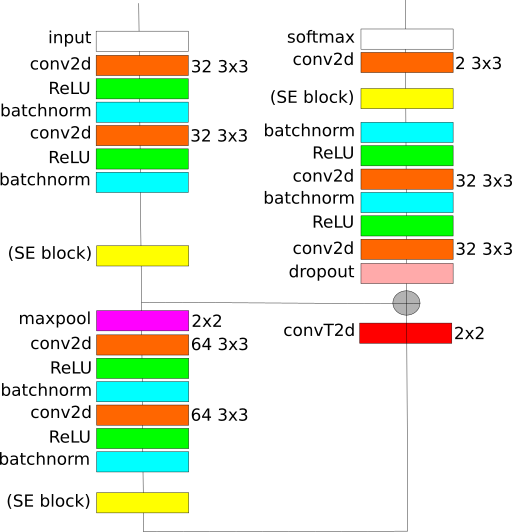
\includegraphics[height=7cm]{images/model_architecture.png}
    \caption{Architecture of our model. The left part depicts an encoder and the right one a decoder. On top of the decoder is also a projection head.}
    \label{fig:model_architecture}
\end{figure}


\subsection{Data Augmentation (DA)}
\label{data-augmentation}

Training deep neural networks usually requires a large amount of data. Since getting enormous quantities of data is commonly expensive, available data should be exploited as much as possible. Data augmentation is a technique that artificially creates new training data from the existing training data. By applying domain-specific transformations of initial data, it generates new training examples that are plausible and depict the same entity. For example, if we rotate an image of a centriole by 90 degrees, the new image still represents a centriole. Applying such transformation makes the model more robust to noise and allows it to generalize better. To improve the performance of our model, we use the following transformations:
\begin{itemize}
    \item The image and corresponding mask are flipped vertically or horizontally, independently with probability $p=0.2$.   
    \item The image is perturbed by adding random Gaussian noise with zero mean and standard deviation of one to each pixel. 
\end{itemize}




\subsection{Squeeze-and-Excitation Block (SE)}
\label{se-block}

Squeeze-and-Excitation blocks \cite{hu2018squeeze} aim to better map the channel dependencies of convolutional layers by accessing global information. They recalibrate outputs of the filters by rescaling channels according to their relative importance.



\subsection{Training Regime}
\label{training-regime}

Due to the high imbalance of the dataset as presented in Section \ref{data-description}, additional measures have to be considered. Without adapting the loss function and balancing the training data, the model might not learn anything. To avoid this problem, Focal Loss \cite{lin2017focal} is employed which mitigates the class imbalance problem. Focal Loss calculates the loss of a single example in the following manner:

\begin{align}
    p_t &= 
    \begin{cases}
     p & \text{if } y = 1  \\
     1 - p & \text{otherwise},
    \end{cases} \\
    FL(p_t) &= -\alpha_t (1 - p_t)^{\gamma}\log(p_t),
\end{align}

\noindent
where $p$ is the prediction of the model, $p_t$ is the confidence of the model in the correct label $y$, and $\alpha$ and $\gamma$  are hyperparameters of the loss. $\alpha$ makes the minority class more important by increasing its loss relatively more than the loss of other classes, while higher values of $\gamma$ punish the model less if its predictions are not so confident.

While Focal Loss certainly helps, the model might still not learn to predict minority class if the imbalance is too high. Since this is the case for our dataset, additional modifications of the training set are required. Instead of inputting the whole image in our model, we rather restrict its view to crops of size $K \times K$. By varying $K$, the trade-off between the size of receptive field, and the imbalance of positive and negative pixels is controlled. Independently of $K$, in the training set are kept only the crops that have at least $pos\_p$ proportion of positive pixels. This way model gets enough information about positive pixels. However, now all training crops contain positive pixels, which is not the case for a random crop. To show the model that there exist also crops without any positive pixels, for each crop in the training set a random crop is added with probability $pos\_p$.




\section{Assignment of Centrioles to Nuclei}
In the beginning, this section explains how the centers of centrioles are found based on the predicted segmentation masks (Section \ref{findings-centers-of-centrioles}). After that, we describe in Section \ref{nuclei-segmentation} how nuclei are segmented and finally, how the centrioles are matched with segmented nuclei. 


\subsection{Finding Centers of Centrioles}
\label{findings-centers-of-centrioles}

\begin{figure}[h!]
    \centering
    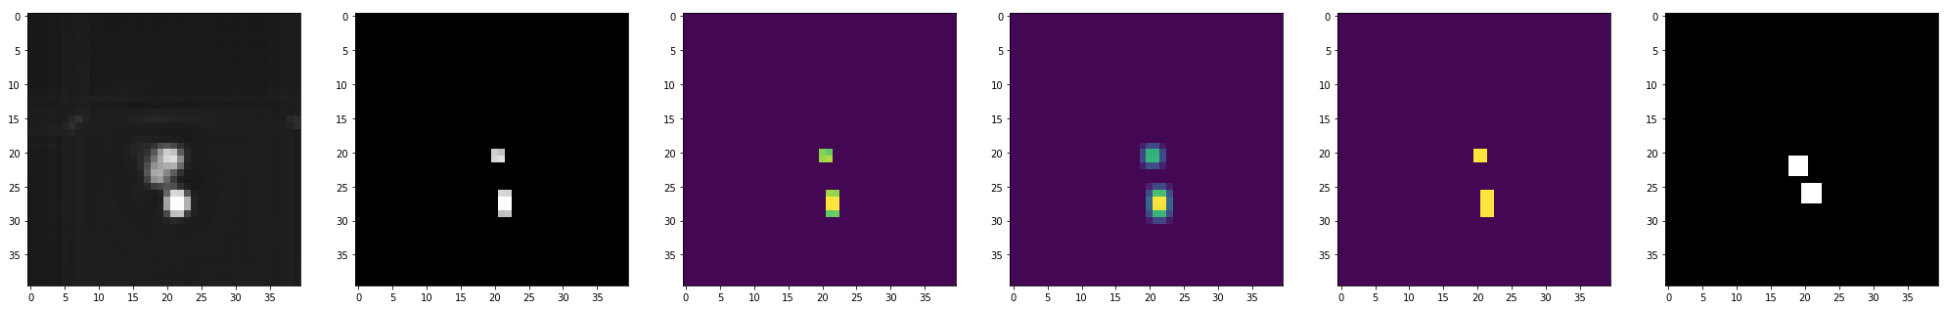
\includegraphics[width=90mm,scale=1]{images/mask_transformations.png}
    \caption{
    Sample images (from left to right): originally predicted segmentation mask, after first global threshold, single-channel result, after Gaussian smoothing, after local mean threshold filter, and ground truth mask.
    }
    \label{fig:transformations}
\end{figure}


From the predicted segmentation masks, centers of centrioles have to be located. This is done in the following manner. First, a global threshold is applied to remove darker blobs while keeping other pixels intact. Then, images are smoothed with a Gaussian kernel to remove noise, and afterwards, a local mean threshold filters the rest of the noise since the majority of the information is located in a small part of the image. After cleaning the mask, contours of each blob are detected to finally locate the centers of centrioles. Figure 2 shows the evolution of the processing step.




\subsection{Semantic Segmentation of Nuclei}
\label{nuclei-segmentation}
We use StarDist \cite{schmidt2018} to segment the nuclei. StarDist is specially made for segmentation of microscopy images. It localizes the nuclei through object detection with star-convex polygons.



\subsection{Matching}
\label{matching}


The assignment of a centriole $c\in\mathbb{C}$ to a nuclei $n\in\mathbb{N}$ is explained in the following procedure (Figure \ref{fig:matching_ex}):
\begin{itemize}
\item Define a graph $G$ with $\mathbb{C}$ and $\mathbb{N}$ as vertices. After calculating distances between all centrioles and nuclei, we create weighted edges $E$ of $G$ if the distance between the nodes is below the threshold $t$.
\item A centriole $c$ inside a nuclei $n$ has a weighted edge $e_{cn}$ of zero. Assign each centriole $c$ with $e_{cn}=0$ to $n$. Then, remove the edge $e_{cn}$ and $c$ from the graph $G$.
\item Assign every centriole $c$ with only one edge to the neighboring nucleus $n$, remove the edge $e_{cn}$ and $c$ from the graph $G$.
\item Each nucleus can have at most four centrioles assigned to it. Break up the assignments of $c$ to $n$ with the longest distance if the nucleus $n$ has more than four edges. These centrioles will not be matched, therefore, remove their vertices and edges. Also, remove vertices and edges for $n$ in $N$, as $n$ cannot be matched anymore if four centrioles are assigned to it. 
\item On the resulting graph $G$, find minimum weight bipartite matching. As a nucleus can match up to four centrioles, add for every $n$: (4 – \#(assigned centrioles)) vertices with the same neighbors.
\item From the resulting matching matrix read the assignments.
\end{itemize}

\begin{figure}[h!]
    \centering
    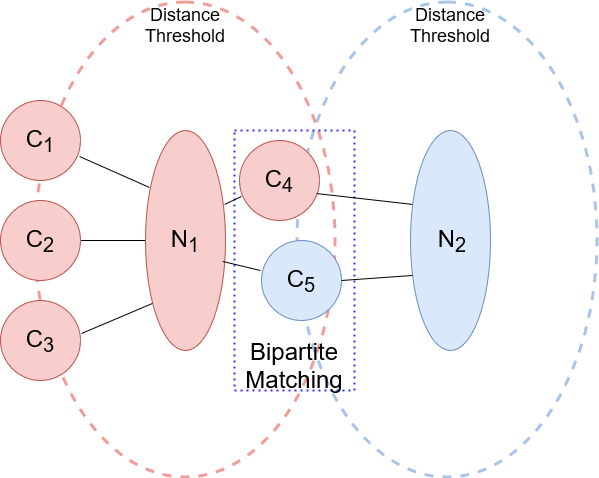
\includegraphics[width=50mm,scale=0.5]{images/Matching.png}
    \caption{Example of matching: centrioles in the threshold with only one edge or inside a nucleus are directly assigned to the nuclei, while the others are assigned with bipartite matching.
    }
    \label{fig:matching_ex}
\end{figure}

Comparing different matching procedures in Figure \ref{fig:matching_comp} to ours, we can see that our procedure connects centrioles and nuclei better. While bipartite matching would minimize the global distance and assign centriole $C_{1}$ to $N_{2}$, the shortest distance matching leaves $C_{5}$ unassigned. As $N_{1}$ has already four assigned centrioles, our matching resolves this problem. The main advantage of our approach is that it first fixes the trivial assignments, and after that, it starts to optimize minimal global distance by bipartite matching. Our proposed approach is completely unsupervised and can be applied even when there are no labels.

\begin{figure}[h!]
    \centering
    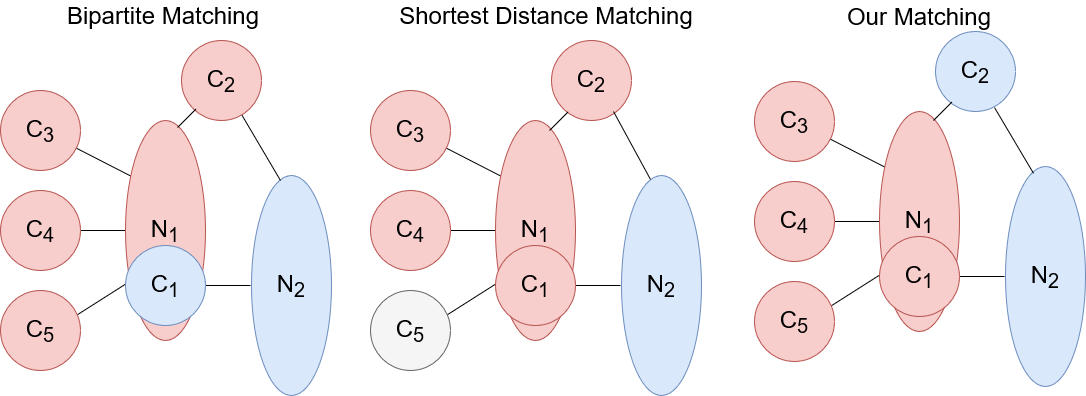
\includegraphics[width=85mm,scale=0.5]{images/compare_matching.png}
    \caption{Comparing different matching procedures: bipartite matching, shortest distance matching from centriole to nuclei and our procedure. Assume a centriole is within the nucleus' distance threshold if an edge exists.
    }
    \label{fig:matching_comp}
\end{figure}



\section{Results}

In this section we present experimental settings and results for semantic segmentation of centrioles (Section \ref{results-segmentation-centrioles}), detection of centers of centrioles (Section \ref{results-detecting-centers}), nuclei segmentation, and assignment of centrioles to nuclei (Section \ref{results-assignment}). Experiments were implemented with help of Pytorch \cite{pytorch}, OpenCV \cite{opencv}, NumPy \cite{numpy}, SciPy \cite{scipy}, and Shapely \cite{shapely} libraries. 



\subsection{Semantic Segmentation of Centrioles}
\label{results-segmentation-centrioles}

To assess our approach and its components, we perform multiple experiments. Each experiment is evaluated on different versions of the model where some components are absent, and on both datasets. Moreover, for the single-channel dataset, we also provide a baseline that is based on standard computer vision techniques. 


\paragraph{Baseline}
As a baseline, we apply the same methods that were used to detect centers of centrioles from predicted masks in Section \ref{findings-centers-of-centrioles}. However, this time the methods take as input the original image and not the predicted masks. The baseline is introduced to motivate why it is even worth using more complicated neural network approaches over simple computer vision methods.


\paragraph{Experimental setting}
We compare three versions of the model: full model, model without Squeeze-and-Excitation block, and model without data augmentation. All models are trained for $40$ epochs, with batch size of $256$, Adam optimizer \cite{kingma2015adam}, initial learning rate of $10^{-5}$, weight decay of $10^{-4}$, dropout of $0.1$, and Focal Loss hyperparameters $\alpha=0.005$ and $\gamma=1.5$. During training, the learning rate is modified according to polynomial learning rate policy \cite{mishra2019polynomial}. All models have the same architecture that is depicted in Figure \ref{model-architecture} (with exception of Squeeze-and-Excitation block in one of them). 
Datasets are first split into the training, validation, and test set according to $80/10/10$ split (e.g. 80\% of instances are in the training set). For the single-channel dataset, the initial training set is then transformed in a set of crops of size $32\times 32$ with more than $pos\_p = 0.02$ proportion of positive pixels. The same is done for the all-channel dataset with $pos\_p = 0.14$. All these hyperparameters were selected by experimentation on a fraction of the dataset by fine-tuning each hyperparameter separately. For the baseline, the size of both kernels is set to 3. 

\paragraph{Evaluation}
When evaluating the models we are principally interested in performance on positive pixels. Therefore, we decided to compare models according to Intersection over Union (IoU), F1-score, precision, and recall. Since all these metrics require binary predictions, predictions of the models are thresholded with the threshold of $0.5$. Results are reported for the best version of each model considering validation F1-score. Due to computationally very demanding training, each experiment is performed only once, however, training, validation, and testing set are fixed across all experiments.


In Table \ref{segmentation-all-channel} are shown results for the all-channel dataset. We can observe that data augmentation has the biggest influence on performance -- without it, IoU score drops by 4\%. This is expected since data augmentation makes the model more robust to noise. More surprising is that Squeeze-and-Excitation blocks harm the performance. While the exact reason is unknown to us, we hypothesize that Squeeze-and-Excitation blocks focus more on obtaining more positive pixels which increases recall but decreases precision. Results for the all-channel dataset (Table \ref{segmentation-all-channel}) as well as results for the single-channel dataset (Table \ref{segmentation-single-channel}) support this claim.

While predicted segmentation masks for the all-channel dataset are great, they are not very helpful for counting individual centrioles. The problem is that annotations are not consistent across channels -- there is a few pixel difference so neighboring centrioles are merged. Nevertheless, the approach is excellent for segmenting centrosomes. Luckily, annotations within a single channel are accurate enough hence the single-channel dataset is utilized for counting centrioles. Relative performance of the neural models is the same as for the all-channel dataset. However, all scores are lower for more than $20\%$ -- it is much harder to segment centrioles only from a single channel. Therefore, we recommend annotating channels jointly as produced segmentations are more accurate. It can also be noticed that the baseline model performs $\approx 20\%$ worse than neural models on the single-channel dataset so use of neural models is well justified.


\begin{table}[h!]
  \caption{Results of semantic segmentation of centrioles on the all-channel dataset.}
  \label{segmentation-all-channel}
  \centering

  \begin{tabular}{cccccc}
    \toprule
    \multicolumn{2}{c}{\textbf{Model components}} & \multicolumn{4}{c}{\textbf{Results}}  \\
    DA & SE & IoU & Precision & Recall & F1-score \\
    \midrule
    \cmark & \xmark & \textbf{0.6680} & \textbf{0.7380} & 0.8757 & \textbf{0.8010} \\
    \cmark & \cmark & 0.6413 & 0.6856 & \textbf{0.9085} & 0.7815 \\
    \xmark & \cmark & 0.6282 & 0.6759 & 0.8990 & 0.7717 \\    \bottomrule
  \end{tabular}
\end{table}

\begin{table}[h!]
  \caption{Results of semantic segmentation of centrioles on the single-channel dataset.}
  \label{segmentation-single-channel}
  \centering

  \begin{tabular}{cccccc}
    \toprule
    \multicolumn{2}{c}{\textbf{Model components}} & \multicolumn{4}{c}{\textbf{Results}}  \\
    DA & SE & IoU & Precision & Recall & F1-score \\
    \midrule
    \cmark & \xmark & \textbf{0.4089} & \textbf{0.5231} & 0.6518 & \textbf{0.5804} \\
    \cmark & \cmark & 0.4015 & 0.4826 & \textbf{0.7049} & 0.5730 \\
    \xmark & \cmark & 0.3662 & 0.4501 & 0.6628 & 0.5361 \\   
    \midrule
     \multicolumn{2}{c}{Baseline} & 0.2094 & 0.2585 & 0.5245 & 0.3464 \\
    \bottomrule
  \end{tabular}
\end{table}


\subsection{Detection of Centers of Centrioles}
\label{results-detecting-centers}

\paragraph{Experimental setting}
To set the global threshold, we tried all integer thresholds in $[0, 255]$ and select the one which gives the best ratio between precision and recall. Finally, we selected the threshold of $180$. We use smoothing with a Gaussian kernel of size 3. The same size is also utilized for the local mean threshold. Additionally, local mean filter subtracts constant $C = -10$ from the mean. Centrioles are not a single pixel, but rather $3\times 3$ patches in the image. Thus, we assume that a centriole is detected if the ground truth centriole is not more than 3 pixels away from the prediction according to Euclidean distance. After using those parameters and transformations, we achieved recall and precision score of $0.85$. Note that for a different threshold we can get up to $0.935$ recall but with only $0.566$ precision, resulting in many false negatives.


\subsection{Assignment of Centrioles to Nuclei and Semantic Segmentation of Nuclei}
\label{results-assignment}


\paragraph{Experimental setting}
The distance threshold in the matching procedure is set to $30$. 
StarDist segments only nuclei with confidence higher than $65\%$, all other settings are kept default. As seen in the left image Figure \ref{fig:cen_nuc_match} some detected centrioles (in red, to the left) are not assigned and must be assumed to belong to another nucleus outside the image.

StarDist sometimes performs very well but sometimes it fails horribly. On the images shown in \ref{fig:cen_nuc_match} the segmentation is very good, but given a bright image, StarDist would find too many nuclei. Our matching performs considerably better than the compared methods of shortest distance and only bipartite matching. However, sometimes mistakes 
still happen. In the right image of Figure \ref{fig:cen_nuc_match} there are two centrioles right next to each other assigned to different nuclei (brown and cyan). This is incorrect as centrioles in pairs normally belong to the same nucleus. As the assignment labels are not provided, we can not evaluate our assignment approach quantitatively. More examples are shown in \ref{sec:appendix}. 

\begin{figure}[h!]
    \centering
    
        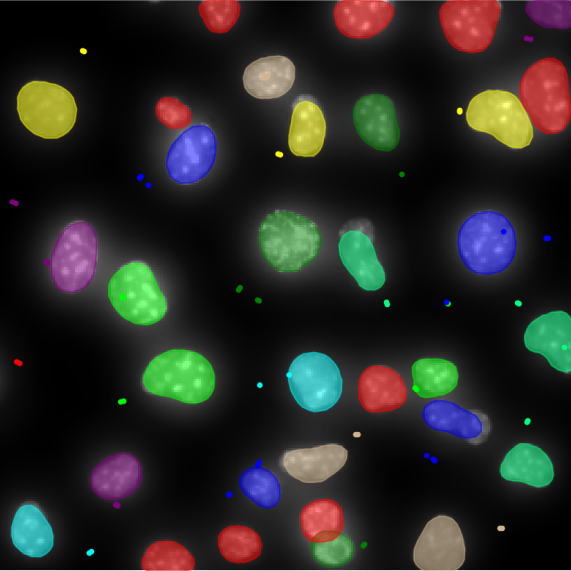
\includegraphics[width=0.45\linewidth]{images/Matching1.png}
        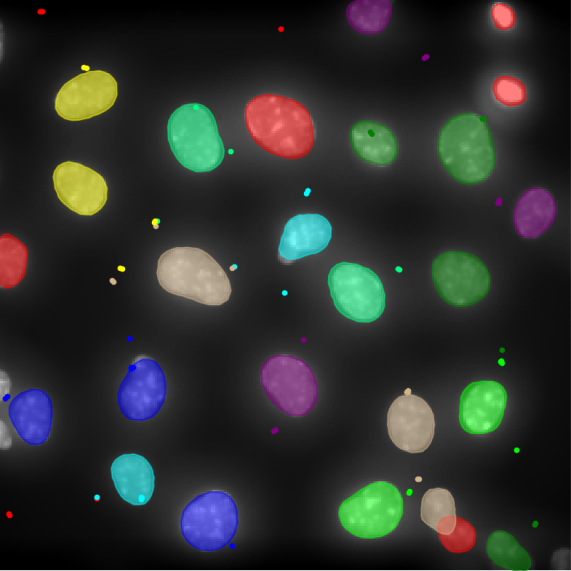
\includegraphics[width=0.45\linewidth]{images/Matching2.png}
    \caption{
    Examples of nuclei segmentation, centriole detection, and matching of those. The colors correspond to their matching, while red nuclei and centrioles are not matched.
    }
    \label{fig:cen_nuc_match}
\end{figure}



\section{Conclusion}

The aim of the paper is to count centrioles and assign them to nuclei. We first present our U-Net-based approach for semantic segmentation of centrioles. It performs well on the single-channel dataset and even better on the all-channel dataset. This is important since the single-channel dataset is used for segmentation of centrioles, while the all-channel dataset contains information about centrosomes. Then, we segment nuclei by employing StarDist, a well-known nuclei segmentation tool. Finally, centrioles are assigned to nuclei by an approach that is a combination of minimum weight matching in a bipartite graph and greedy matching. By combining the advantages of bipartite and greedy matchings, it outperforms both of them separately.

\pagebreak

\bibliographystyle{IEEEtran}
\bibliography{literature}

\clearpage
\section{Appendix}
\label{sec:appendix}
\subsection{Nuclei segmentation of StarDist}
Figure \ref{fig:seg_nuc} shows examples of the nuclei segmentation of StarDist. On the left image, it performs well, while segmentation on the right one is poor.

\begin{figure}[h!]
    \centering
    
        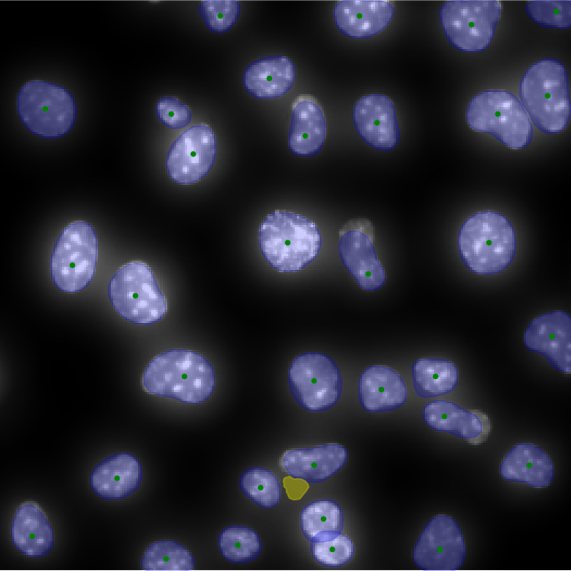
\includegraphics[width=0.45\linewidth]{images/NucSeg1.png}
        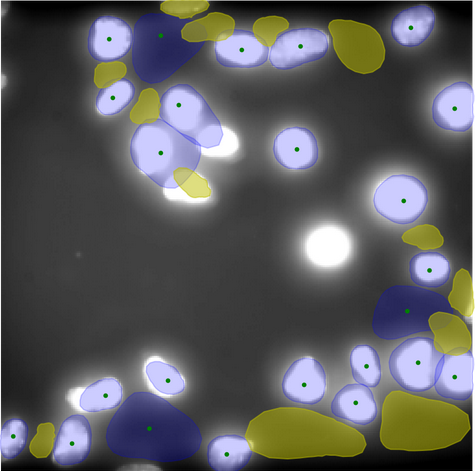
\includegraphics[width=0.45\linewidth]{images/Nuc_seg.PNG}
    \caption{
    Examples of nuclei segmentation. Yellow nuclei are filtered out by the probability threshold of 65\%.
    }
    \label{fig:seg_nuc}
\end{figure}

\subsection{Centriols over ground truth}
The Figure \ref{fig:cen_gt} below displays two examples of centriole predictions, in red, and the ground truth centrioles, in blue, on one image.
\begin{figure}[h!]
    \centering
    \begin{tabular}{cc}
        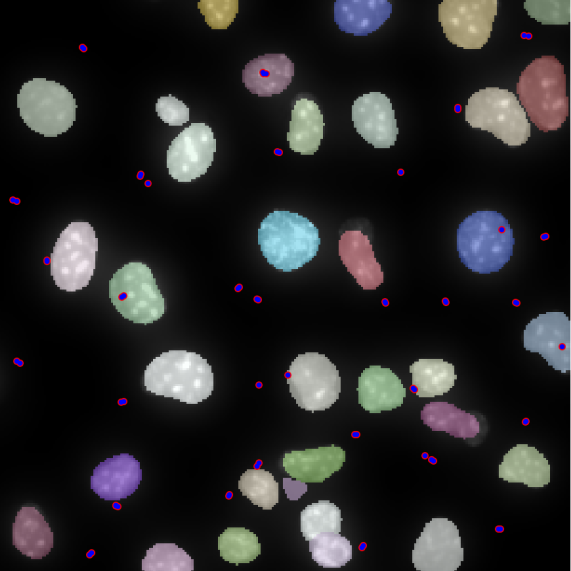
\includegraphics[width=0.65\linewidth]{images/GTonPred.png}
        \\
        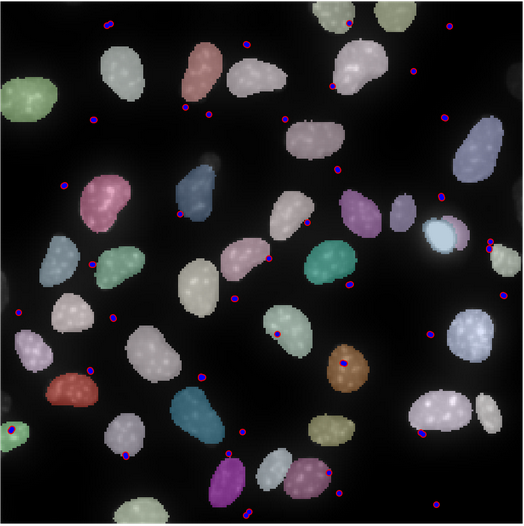
\includegraphics[width=0.65\linewidth]{images/GT2.PNG}
        
    \end{tabular}
    \caption{
    Predicted centrioles (red) and the ground truth centrioles (blue).
    }
    \label{fig:cen_gt}
\end{figure}

\subsection{Comparison matching}
This Figure \ref{fig:app_match_comp} illustrates a simple example when a bipartite only matching procedure and ours result in different matching. Bipartite only matching matches the centriole that is inside another nucleus incorrectly. 
\begin{figure}[h!]
    \centering
        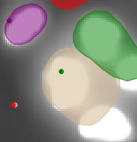
\includegraphics[width=0.35\linewidth]{images/bip_matching.PNG}
        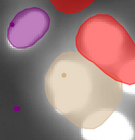
\includegraphics[width=0.35\linewidth]{images/our_matching.PNG}
        
    \caption{
    Bipartite matching on the top and our matching on the right. Our matching performs better.
    }
    \label{fig:app_match_comp}
\end{figure}
\end{document}